\chapter{Plugins per Fiji}
\label{chap:plugins}
\noindent Cosa è \textit{``Fiji''}? Come è nato? Quali sono le differenze con \textit{ImageJ} e come si sviluppa un plugin per l'applicativo preso in esame? Queste sono le principali domande a cui daremo risposta in questo capitolo.

\section{ImageJ}
\noindent \textit{``ImageJ''} è stato sviluppato nel 1997 dal \textit{NIH} (\textit{``National Institutes of Health''}). È un software open-source sostenuto da una vasta community di sviluppatori e ricercatori e oggi ed uno dei software più utilizzati da medici e biologi a fini scientifici.
È conosciuto all'interno della lista di distribuzioni ad esso collegate come \textit{``ImageJ 1.x''} o, per brevità IJ1. L'ultima versione risale al 31 marzo 2022 (\textit{1.53q}), ma al giorno d'oggi ancora attivo e ampiamente scaricato. È considerato un tool capace di adattarsi alla maggior parte dei problemi legati all'analisi di immagini, ed è per questo usato sia nel campo della microscopia che ad esempio in quello della scienza dei materiali. La libreria che lo compone è accessibile via API, permettendo a sviluppatori del settore di riusarne e estenderne le funzionalità attraverso la creazione di \textit{Plugin}, e di registrare \textit{Macro} automatizzando processi interni attraverso linguaggi come Java, Beanshell, Javascript e una DSL (\textit{Domain Specific Language}) per IJ1. L'utilizzo delle Macro permette ad utenti non Computer Scientists di non dover seguire un percorso di apprendimento particolare per l'automatizzazione di specifici workflow~\cite{Schneider2012}.

\section{Differenze tra ImageJ2 e ImageJ 1.x}
\noindent La seguente tabella è proveniente dalla fonte~\cite{CheatSheet} e non è stata tradotta in lingua italiana per evitare incomprensioni.
\begin{table}[H]
\begin{tabularx}{\textwidth}{|l|X|X|}
\hline
\small{} &
\small{ImageJ 1.x} & 
\small{ImageJ2} \\
\hline
Image types & uint8, uint16, float32, rgb &	bit, uint2, uint4, uint8, uint12, uint16, uint32, uint64, uint128, int8, int16, int32, int64, float32, float64, cfloat32, cfloat64, bigint, bigdec, argb, <your-image-type-here> \\
\hline
Plugin types & PlugIn, PlugInFilter, PlugInTool & Command, Op, Tool, IOPlugin, Service, Converter, Codec, Format, DataHandle, TextFormat, ScriptLanguage, Display, UserInterface, Platform, App, Gateway, ModulePreprocessor, ModulePostprocessor, CodeRunner, ..., <your-plugin-type-here> \\
\hline
Dimensions & 5D—XYZCT &	N-dimensional—X, Y, Z, time, channel, emission spectra, lifetime, cell polarity, <your-dimension-here> \\
\hline
Image formats & HandleExtraFileTypes & SCIFIO—including Bio-Formats plugin; <your-format-here> \\
\hline
Parameters & GenericDialog & SciJava module @ parameter syntax—callable from ImageJ, KNIME, OMERO, CellProfiler, ..., <your-tool-here> \\
\hline
Script languages & IJ1 macro, JavaScript, BeanShell, Java &	BeanShell, Clojure (Lisp), Groovy, Java, JavaScript, JRuby, Jython (Python), Renjin (R), Scala, <your-language-here>\\
\hline
User interface & AWT & Legacy, Swing, AWT, Apache Pivot, Eclipse SWT, JavaFX, KNIME, CellProfiler, OMERO, <your-ui-here> \\
\hline
Distribution & Download, install and update manually & Hundreds of update sites; receive updates automatically (when you want!) \\
\hline
\end{tabularx}
\end{table}

\section{ImageJ2}
\noindent Il progetto \textit{``ImageJ2''} è nato nel 2009 ed è stato costruito su \textit{SciJava Common} che ne rappresenta il core. È il vero successore di \textit{ImageJ} 1.x. La libreria è stata infatti riscritta, ripensata e totalmente ridisegnata, facilitando l'estensibilità di tutti i tipi di dato. Segue i dettami dei principi \textit{SOLID} separando i compiti, disaccoppiando l'UI dal dominio applicativo, enfatizzando così la possibile integrazione con qualsiasi applicazione e/o libreria e portando il progetto ad essere interoperabile. Si può infatti intendere il progetto come un framework condiviso per l'elaborazione d'immagini attraverso il quale si può scrivere una sola volta il codice per eseguirlo su diversi applicativi come \textit{KNIME}, \textit{CellProfiler}, \textit{OMERO} e \textit{Icy}. La compatibilità verso la prima versione è una delle principali feature di cui dispone e ciò permette una facile migrazione agli sviluppatori tramite la libreria \textit{ImageJ Legacy}. È provvisto anche della libreria \textit{ImageJ Updater} per fare l'aggiornamento di ogni singolo plugin della libreria \textit{Imagej Ops} che comprende una serie di algoritmi di elaborazione immagini riusabili e di \textit{ImageJ Common} che usa \textit{``ImgLib2''} ed il core del modello dei dati delle immagini.
Infine per la maggior parte delle operazioni di I/O fa uso della libreria \textit{SCIFIO} (\textit{``SCientific Image Format Input and Output''})~\cite{https://doi.org/10.1002/mrd.22489}~\cite{Rueden2017}~\cite{Hiner2016}~\cite{10.1093/bioinformatics/bts543}.


\section{Fiji}
\noindent È l'acronimo per \textit{Fiji is Just ImageJ}. L'architettura nasconde al suo interno la libreria \textit{ImageJ2} e fornisce un'estensiva lista di plugin forniti di default.
L'obiettivo principale di Fiji è migliorare l'esperienza utente dei ricercatori che non hanno conoscenze legate alla programmazione. I plugin forniti sono nella quasi totalità provvisti di una documentazione estensiva, dove si è guidati sia a livello generale con una prima panoramica delle funzionalità, sia a livello specifico in tutorial e dataset scaricabili. Il successo e la popolarità di \textit{Fiji} è dato anche dalla sua capacità di integrarsi per operazioni e compiti troppo onerosi per l'applicazione con applicativi terzi. \textit{Fiji} si interfaccia inoltre con MATLAB e \textit{ITK}, e attraverso \textit{ImgLib} e \textit{ImageJ2} e permette l'adozione di ogni piattaforma scritta in Java~\cite{Schindelin2012}.


\section{Sviluppo di un plugin}

\subsection{Primi passi}
\noindent Prima di tutto si deve creare un progetto Java con un IDE a piacimento (\textit{``IntellJ IDEA''} o \textit{``Eclipse''} ad esempio) e creare un file pom.xml all'interno della radice del progetto. Per vedere un esempio pratico di questo osservare \textit{UnibosDS4H/DS4H} oppure \textit{imagej/example-imagej2-command}.

\begin{listing}[H]
\begin{minted}{xml}
<?xml version="1.0" encoding="UTF-8"?>
<project xmlns="http://maven.apache.org/POM/4.0.0"
...
<modelVersion>4.0.0</modelVersion>
<groupId>DS4H-Image-Alignment</groupId>
<artifactId>DS4H-Image-Alignment</artifactId>
<version>1.0.4</version>
<parent>
    <groupId>org.scijava</groupId>
    <artifactId>pom-scijava</artifactId>
    <version>25.0.0</version>
    <relativePath />
</parent>
<repositories>
    <repository>
        <id>imagej.public</id>
        <url>http://maven.imagej.net/content/groups/public</url>
    </repository>
</repositories>
    <dependencies>
        <dependency>
            <groupId>net.imagej</groupId>
            <artifactId>imagej</artifactId>
        </dependency>
    </dependencies>
</project>
\end{minted}
\caption{Esempio parziale di file pom.xml UnibosDS4H/DS4H su Github} \label{lst:pom}
\end{listing}

\subsection{Il codice sorgente}
\noindent Si può scegliere di usare ImageJ2 o ImageJ 1.x, il quale viene tradotto automaticamente tramite un componente interno chiamato \textit{``Java Assist''}. Il primo esempio (\Cref{lst:ImageJ2}) è quello consigliato al momento ed è la via preferibile, mentre il secondo esempio (\Cref{lst:ImageJ1} e~\Cref{lst:ImageJ1Config}) è la versione Legacy che si può usare senza temere ma non permette di sfruttare le ultime features.

\begin{listing}[H]
\begin{minted}{java}
package hello;

import org.scijava.command.Command;
import net.imagej.ImageJ;

@Plugin(type = Command.class)
public class HelloWorld implements Command {
    /**
        * Main method is actually used only for debugging
        **/
    public static void main(final String... args) {
        final ImageJ ij = new ImageJ();
        ij.launch(args);
        ij.command().run(HelloWorld.class, true);
    }
    @Override
    public void run() {
        // ...
    }
}
\end{minted}
\caption{Esempio semplice di un plugin Fiji in cui si fa uso di ImageJ2} \label{lst:ImageJ2}
\end{listing}
    
\begin{listing}[H]
\begin{minted}{java}
package hello;

import ij.IJ;
import ij.plugin.PlugIn;

public class HelloWorld implements PlugIn {
    @Override
    public void run(String s) {
    	// ...
    }
}
\end{minted}
\caption{Esempio semplice di un plugin Fiji in cui viene utilizzato ImageJ 1.x} \label{lst:ImageJ1}
\end{listing}

\begin{listing}[H]
\begin{minted}{text}
	Plugins>Hello, "Hello World", hello.HelloWorld
\end{minted}
\caption{Esempio di file plugins.config obbligatorio nel caso dell'uso di ImageJ 1.x} \label{lst:ImageJ1Config}
\end{listing}

\subsection{Transizione da ImageJ 1.x a ImageJ2}
\noindent Per chi ha già esperienza con la prima versione, qui può trovare una cheat sheet utile per effettuare la transizione alla seconda \Cref{fig:6} e \Cref{fig:7}.

\begin{figure}[H]
\centering
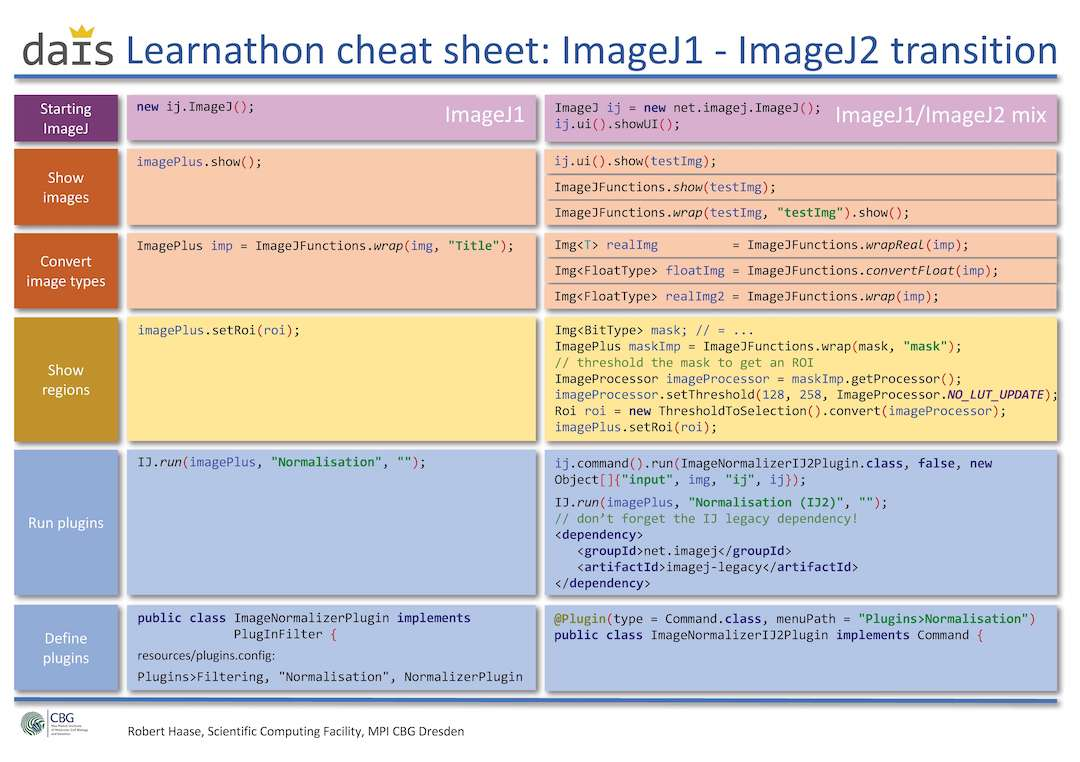
\includegraphics[scale=0.4,keepaspectratio]{ij_legacy_cheetsheet_Pagina_1.jpg}
\caption{Pagina 1, di Robert Haase, Scientific Computing Facility, MPI CBG Dresden}
\label{fig:6}
\end{figure}

\begin{figure}[H]
\centering
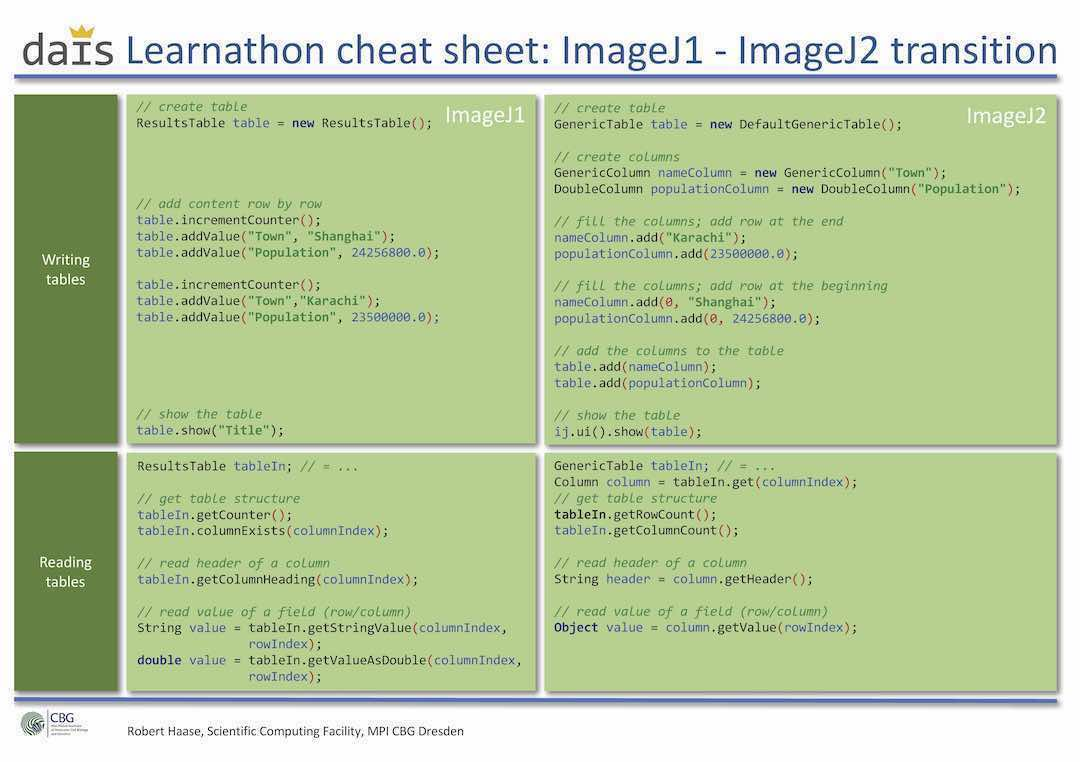
\includegraphics[scale=0.4,keepaspectratio]{ij_legacy_cheetsheet_Pagina_2.jpg}
\caption{Pagina 2, di Robert Haase, Scientific Computing Facility, MPI CBG Dresden}
\label{fig:7}
\end{figure}


\subsection{Build}
\noindent All'interno del file pom.xml dev'essere presente una parte di codice per eseguire il processo di creazione del file JAR, una di queste permette di includere agli assets \Cref{lst:build}.

\begin{listing}[H]
\begin{minted}{xml}
<build>
	<resources>
        <resource>
            <directory>src/main/assets</directory>
            <includes>
                <include>**/*</include>
            </includes>
        </resource>
    </resources>
</build>
\end{minted}
\caption{pom.xml, sottosezione build}\label{lst:build}
\end{listing}

\noindent Per creare il file JAR nella giusta cartella occorre creare, se non già presente in questo percorso
\textbf{HOME/.m2}, un file chiamato \textbf{settings.xml} come mostrato in \Cref{lst:scijavadir}

\begin{listing}[H]
\begin{minted}{xml}
<settings>
    <profiles>
        <profile>
            <id>imagej</id>
            <activation>
                <file>
                    <exists>${env.HOME}/Desktop/Fiji.app</exists>
                </file>
            </activation>
            <properties>
                <scijava.app.directory>${env.HOME}/Desktop/Fiji.app </scijava.app.directory>
            </properties>
        </profile>
    </profiles>
</settings>
\end{minted}
\caption{settings.xml valido per Fiji}\label{lst:scijavadir}
\end{listing}

\noindent Come compilare un file Maven dipende dall'IDE di riferimento. In questo paragrafo spiegheremo come si fa con \textit{IntellJ IDEA}, il quale fornisce tre modalità. La prima è tramite Run → Edit Configurations -> Maven, la quale non ha bisogno normalmente di specifici comandi per l'inizializzazione, e permette una volta eseguito di creare il file JAR. La seconda modalità è attraverso il plugin stesso, mostrato in \Cref{fig:8}, dove l'UI permette agli utenti meno esperti di usufruire dei comandi e dei profili Maven senza avere conoscenze pregresse.

\begin{figure}[H]
    \centering
    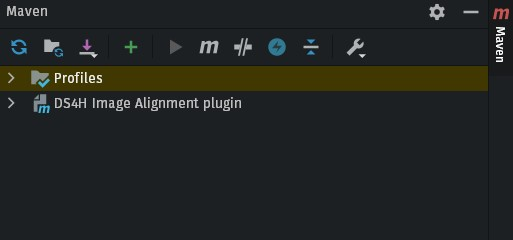
\includegraphics[scale=1,keepaspectratio]{plugin_maven_idea.jpg}
    \caption{Esempio plugin Maven IntelJ IDEA}
    \label{fig:8}
\end{figure}

\noindent L'ultima modalità è quella di digitare i comandi specifici direttamente dal terminale, ad esempio \Cref{lst:mvn}:

\begin{listing}[H]
\begin{minted}{bash}
    mvn clean & mvn compile & mvn install
\end{minted}
\caption{Esempio per pulire, compilare e creare il file JAR}\label{lst:mvn}
\end{listing}

\subsection{Service}
\noindent A differenza di \textit{ImageJ 1.x}, dove per accedere alla maggior parte delle sue funzionalità si usano dei metodi statici, per \textit{ImageJ2} ogni parte ha la sua logica di business incapsulata in un servizio. Un servizio non è altro che una classe con una serie di responsabilità legate ad un solo argomento. \textit{ImageJ2} dispone di tantissimi Service, tra questi possiamo ricordare:
\begin{itemize}
    \item AppService - tiene traccia l'applicazione presente nel contesto.
    \item DisplayService - tiene traccia delle schermate disponibili, di quella attiva, e da l'abilità di crearne di nuove.
    \item EventService - gestisce gli eventi legati all'applicazione, ed è la base per gestire la comunicazione tra le diverse parti dell'applicativo.
    \item IOService - contiene gli strumenti per aprire e salvare file all'interno del contesto.
    \item MenuService - ha la struttura del menu dell'app che può essere costruita attraverso questo servizio.
    \item ModuleService - tiene traccia dei moduli disponibili, e fornisce l'infrastruttura per eseguirli.
    \item ObjectService - tiene traccia degli oggetti disponibili, inclusi i Datasets e i Displays.
    \item OptionsService - ha gli strumenti per gestire le impostazioni del programma.
    \item PlatformService - provvede hooks per estendere l'applicativo rispetto al sistema operativo in uso.
    \item PluginService - tiene traccia dei plugins, e fornisce gli strumenti per eseguirli.
    \item ScriptService - permette di eseguire gli script e macro.
    \item StatusService - tiene traccia dello stato delle operazioni in corso.
    \item ThreadService - gestisce multithreading, utile per eseguire più operazioni e task in parallelo.
    \item UIService - esegue le UI per interagire con ImageJ.
    \item DatasetService - ha gli strumenti per creare e gestire i dati delle immagini.
    \item ImageDisplayService - simile a DisplayService, ma per gli ImageDisplays.
    \item OverlayService - ha gli strumenti per creare e gestire gli overlays e le ROIs delle immagini.
    \item FormatService - servizio per gestire i formati delle immagini disponibili.
\end{itemize}
    


\subsection{Consigli}
\noindent La fase più importante per la creazione di software è la quella di progettazione del dominio e della business logic. È importante non pensare alle librerie che si useranno, poiché rappresentano una parte terza che dev'essere sempre possibile cambiare, ad esempio se si sceglie una differente libreria di UI durante la fase di sviluppo rispetto a quella già implementata, la modifica si deve poter fare senza dover cambiare parti del dominio. È buona pratica studiare il linguaggio usato, conoscere cosa si intende per OOP e cosa sono i principi SOLID.